\section{Introduction}
\begin{frame}{Introduction}
\end{frame}

% **************************************************
% HIGH-PERFORMANCE COMPUTING
% **************************************************
\subsection*{High-performance computing}
\begin{frame}{High-performance computing}

\begin{itemize}\pause
\item Increasing need for computational power\pause
\item Grids and cloud computing\pause
\item Many-core systems\pause
\item Many computations running on high-performing systems do not make
  use of the performance available.\pause
\item We need software that achieves \emph{strong scaling}.
\end{itemize}
\end{frame}


% **************************************************
% COPERNICUS
% **************************************************
\subsection*{Copernicus}
\begin{frame}{Copernicus}{What is Copernicus?}

\begin{itemize}\pause
\item Copernicus is a software system that was originally made to
  distribute and parallelize large molecular simulations.\pause
\item It's adopts a server-client model.
\end{itemize}

\pause

\begin{center}
  \phantom{\includegraphics<1-3>[width=0.5\textwidth]{gfx/architecture.pdf}}
  \includegraphics<4>[width=0.5\textwidth]{gfx/architecture.pdf}
\end{center}
\end{frame}


\begin{frame}{Copernicus}{What is Copernicus?}
\begin{itemize}\pause
\item Instances communicates in a peer-to-peer network.\pause
\item It shares attributes with cloud computing.
\end{itemize}

\pause

\begin{center}
  \phantom{\includegraphics<1-3>[width=0.5\textwidth]{gfx/peer2peer.pdf}}
  \includegraphics<4>[width=0.5\textwidth]{gfx/peer2peer.pdf}
\end{center}
\end{frame}


\begin{frame}{Copernicus}{Projects}

\begin{itemize}\pause
\item The inputs to Copernicus are data-flow network descriptions.\pause
\item A model of a real-life example would look like this:
\end{itemize}

\begin{center}
  \phantom{\includegraphics<1-3>[width=\textwidth]{gfx/liveexample.pdf}}
  \includegraphics<4>[width=\textwidth]{gfx/liveexample.pdf}
\end{center}

\end{frame}

%\begin{frame}{Copernicus}{Architecture}
%
%\begin{columns}
%  \column{0.5\textwidth} 
%  \begin{itemize}
%  \item An example Copernicus architecture with two project servers
%    and four network servers.\pause
%  \item Clusters 0 and 1 may be located in A with a common gateway
%    server, while cluster 2 is located at B.
%  \end{itemize}
%
%  \column{0.5\textwidth}
%  \begin{figure}
%    \centering
%    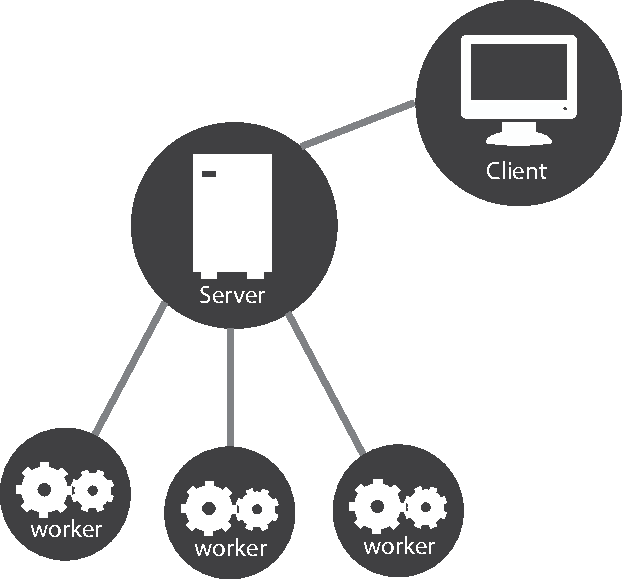
\includegraphics[width=\textwidth]{gfx/architecture.pdf}
%  \end{figure}
%\end{columns}
%
%\end{frame}
%
%
%\begin{frame}[shrink=3]{Copernicus}{Network model}
%\begin{columns}
%  \column{0.5\textwidth}
%  \begin{figure}
%    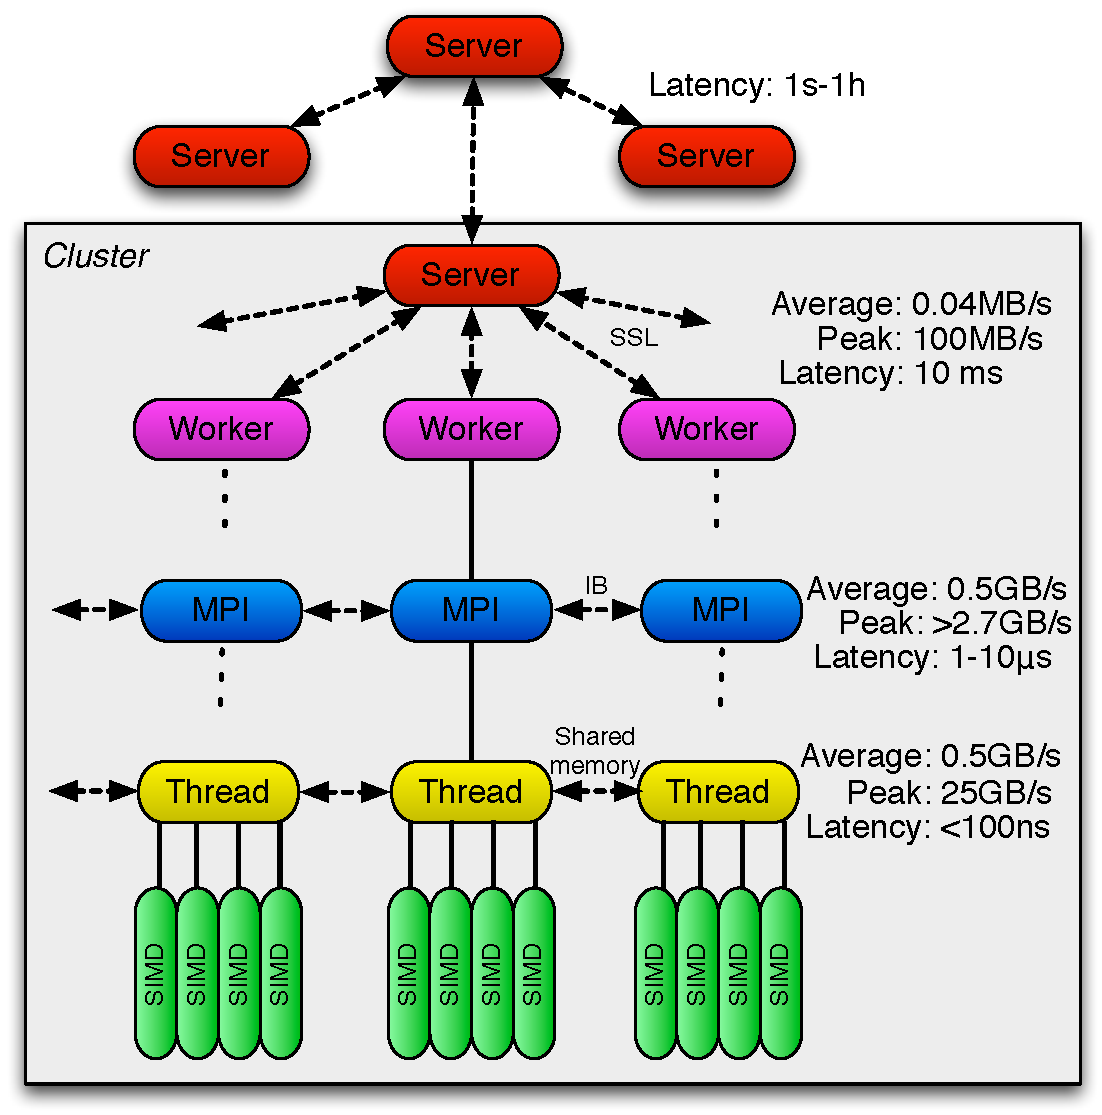
\includegraphics[width=\textwidth]{gfx/parallelization.pdf}
%  \end{figure}
%
%  \column{0.5\textwidth}
%  \begin{itemize}\pause
%  \item The nonbonded kernels use SIMD assembly and each Copernicus
%    task is a massively parallel message-passing simulation.\pause
%
%  \item Beyond the point of efficiently scaling individual
%    simulations, hundreds of workers are employed on a typical cluster
%    or supercomputer, and these communicate with other resources
%    through additional servers.\pause
%
%  \item Top-level servers interact with controllers, or project
%    servers, to determine what tasks to execute.
%  \end{itemize}
%\end{columns}
%\end{frame}


% **************************************************
% PROBLEM STATEMENT
% **************************************************
\subsection*{Problem statement}
\begin{frame}{Problem statement}

\begin{itemize}\pause
\item The aim of our project was to design a suitable input
  description-language for Copernicus.\pause

\item Intuitive language targeted at users familiar with, but not
  necessarily adept at, programming.\pause

\item A language that is easy to extend with a graphical interface.
\end{itemize}

\end{frame}
